\documentclass[acmlarge]{acmart}

\usepackage{booktabs} % For formal tables
\usepackage{mathtools}
\usepackage{graphicx}
\usepackage{amsmath}
\usepackage{wrapfig}
\usepackage{hyperref}


\usepackage[ruled]{algorithm2e} % For algorithms
\renewcommand{\algorithmcfname}{ALGORITHM}
\SetAlFnt{\small}
\SetAlCapFnt{\small}
\SetAlCapNameFnt{\small}
\SetAlCapHSkip{0pt}
\IncMargin{-\parindent}
\settopmatter{printacmref=false}
\setcopyright{none}

\makeatletter
\let\@authorsaddresses\@empty
\makeatother


% Document starts
\begin{document}
% Title portion
\title{Fairness, Equality, and Equity: Algorithmic Approaches}
\titlenote{Current state and future}

\author{Juan Enrique Stücker Martínez}
\orcid{1234-5678-9012-3456}
\affiliation{%
  \institution{RWTH Aachen University}
  \city{Aachen}
  \country{Germany}}
\email{juan.stuecker@rwth-aachen.de}

%

\begin{abstract}
  Some of the basic needs for a society to function well - as hard as it is to define wellness in a social context - are "fairness", "equality", and "equity" for all the people taking part \textsl{in} the society. Fighting injustice is always a pressing subject in human societies. In the contemporary world expressing concern is now more democratized with access to the internet and in the hands of a bigger section of the population, which makes possible to diversify the topics in public discussion. Despite of this shift, it still is a rather untouched subject to judge and impose standards on algorithms by these 3 basic concepts. This paper will try to define what it means for an algorithm to be fair and for it to enforce equality and or equity. \\
  Today's world is no absent of algorithms whose functionality affects certain groups of people more than others. The technological world has failed in many mainstream services we use in our day-to-day life to reach these goals, but concern has led to some change and a growing motivation for action, both from Academia as well as from the population and the Market itself. As uncomfortable, and even inconvenient as it is, this evolution is necessary.\\
  By describing the mathematical and abstract concepts that attempt to replicate or represent these key themes (Fairness, Equality, Equity), and the ceonceptual problems that result in the creation of these definitions, we can gain a different perspective on how to engage with these difficult problems. Problems that for a long time were mainly approached from the Social and Political Sciences.\\
  More on, not only can Algorithms reach for a moral standard, in some cases they can even help to solve more general social problems in humanity.
  That is what algorithms can be, a double-edged sword.

\end{abstract}

\keywords{Social Problematics, Bias in Algorithms, Fairness}


\maketitle

% The default list of authors is too long for headers.
\renewcommand{\shortauthors}{}

\graphicspath{{../figures/}}

\section{Introduction}

Although a sense of fairness came into question very often in history during the development of mathematical or algorithmic methods, especially on the ones that had the potential to affect people\cite{Phen20}, action has been insufficient. Technology has a lot of examples of unfairness enforcing examples. \\
The moral character of our societies evolves, and constantly changes, algorithms often permeate the social ideals of the time they are developed in, through human developers, and or through the users themselves. Algorithms set a mirror to ourselves, and our society as they reflect amongst other things, our faults. Social standards change\cite{Sewe17}, often for the better, and in today's society, which more openly than before puts pressure to advance those standards, algorithms should also follow through.
\begin{quote}
"The wide variety of sectors in which automated decision-making systems are employed
can have serious repercussions on human rights, whether related to health treatments,
job opportunities, predictive policing or otherwise, rendering the capability to obtain an
effective remedy in each of these is even more essential". -Study on Human Rights Dimensions of Automated Data Processing Techniques, and possible regulatory implications\cite{CommNaN}
\end{quote}
The question of the motivation of the developers then arises. Do they develop an unfair algorithm willingly, and especially conscious of the consequences? The answer is in a lot of cases "no". \cite{OCDK19}
\begin{quote}
  "Never attribute to malice that which is adequately explained by stupidity" -Robert J. Hanlon
 \cite{Bloc81}.
\end{quote}
To not be too harsh with the term, stupidity here suggests \textsl{unaware consequences of the work of the creators of such algorithms}. An unfair algorithm is not always made by unfair people. Frequently used machine-learning generated algorithms depend on the Data available for them. Thus, a big challenge is how to avoid such an outcome. Not only can we and \textsl{must} we analyze algorithms critically, algorithms can also intervene in the solution of social challenges. \\
Approaches to abstract fairness notions in the fields of economics, mathematics, and social choice make able to apply theoretically generated solutions to real-world problems. The very well known Cake-Cutting Problem for division problems is a great example. \\
Ironically, algorithms can be the solution, to algorithmically generated problems, the idea of an algorithm observing and accounting for another algorithm may sound bizarre, but it's the best solution to often very complex functioning systems a human may not be able to rapidly assess. \\
Algorithmic Fairness has been on the radar of many researchers in the past decade, and with the rise of machine-learning methods for both the industry and academia, awareness of the flaws of some algorithms  is increasing, but there is no unified approach to assess, and resolve the imperfections within the systems. Often, definitions of fairness collide with one another, and fairness-controlling methods sometimes drastically change and are even discarded. The absence of a unified approach results in the necessity to observe the whole system for flaws. \\
Throughout this paper, definitions will be the base from which the different approaches, both mathematical as well as conceptual. It is very important to be very clear with the fairness goals for the systems to analyze to avoid conflicts. Fairness definitions can be contradictory with one another in certain circumstances\cite{CPF*17}.
\section{Basic definitions}
The interest of this paper is rather on the mathematical definitions of our three terms, but for a good foundation it will begin with the ones found in the Oxford Dictionary for the English language.
\begin{itemize}
  \item Fairness:
  "The quality of treating people equally or in a way that is right or reasonable"\cite{Fairness}
  \item Equality:
  "The right of different groups of people to have a similar social position and receive the same treatment"\cite{Equality}
  \item Equity:
  "The situation in which everyone is treated fairly and equally"\cite{Equity}\\
  There is often a different interpretation of equity as an extension of equality, where every actor receives a good, based/on proportion on context and characteristics of the agnet."Give everyone what they \textsl{need} to succeed". This functions as a counterpoint to the simpler view of equality where everything is divided into identical parts.
  \item System:\cite{Compsysbias}
  "A set of things working together as parts of a mechanism or an interconnecting network."

  A computer system is a set of integrated devices that input, output, process, and store data and information.
  In this paper, the use of the word system will often refer to the set of components, from mathematical models until applied software that builds the entity performing the activity that was ought to be automated.
\end{itemize}
%recite some actual examples on today's world, this is probably going to be the biggest section fo all
\section{Contemporary problems}

\subsection{Algorithmic Bias}
\label{AlgorithmicBias}

Being biased is usually understood as not having fair treatment, and or not being neutral in a specific situation. Friedman defines a \textsl{Computer System being biased} as \begin{quote}"Systems that systematically and unfairly discriminate against certain individuals or groups of individuals in favor of others"\cite{Compsysbias}.\end{quote} The reason for a transition to algorithmic decision-making is usually effectiveness, efficiency, and a promised form of objectivity. "They are tools for better
applying available information to make real-world decisions with less noise or variance
and without the influence of human subjectivities"\cite{OBS*19}. However, it is realistically impossible to have a completely fair algorithm \footnote{Given the amount of ways how an algorithm may be affected, and the small amount of control in different stages of development.} Despite this, fairness standards, and goals are absolutely necessary.\\
Bias can occur in different parts of the development of an algorithm. The following enlisting uses the classification of Friedman et al.\cite{Compsysbias}

\subsubsection{Preexsitig bias}: \label{PreexsitingBias}
"Preexisting bias has its roots in social institutions, practices, and attitudes"\cite{Compsysbias}
Individuals that have a significant design input to the system may influence the model with personal bias (e.g., listing specifications that embody gender discrimination).
\subsubsection{Technical bias}: \label{TechnicalBias}
Technical constraints, or shortcomings. Does the technology used in the system have limitations that lead to possible unfair outcomes? (e.g not being able to correctly represent a population due to a lack of ways to make a survey; not having the resources to assess the adaptations needed for a sector of a population with disabilities, etc.)
\subsubsection{Emergent bias}: \label{EmergentBias}
Arises upon contact with users of the system, and not before. Having a moldable system, or a system that changes based on user input (e.g every system using feedback from the user to dynamically shape an internal model, such as recommendation systems, etc.)

Every part of the process is then to some extent \textsl{sensitive} to be biased.
The paper will largely focus on the machine-learning context, given that it is the technique that has the most literature on the subject in the last years.\\
In contrast algorithms the are not created without statistical or machine-learning models rely less on inputted data and more on the logic behind the systems. The concept of fairness prevails, but the methods listed below may not be as easily applied.\\
machine-learning algorithms often require a very large Data Set to produce passing solutions, this is the reason why there is a strong relationship between \textsl{Algorithmic Bias}\nameref{AlgorithmicBias} and \textsl{Data Bias}\label{DataBias}, which can be denoted as :
\begin{enumerate}
  \item Data that does not include variables that properly capture the phenomenon we want to predict
  \item Data includes content produced by humans which may contain bias against groups of people
  \item "A systemic distortion in the data that compromises its representativeness” \cite{OCDK19}
\end{enumerate}
\begin{quote}"biased training data results in biased algorithms, which in turn produce more biased data in a feedback loop"\cite{GSC18} \end{quote}
No Data Set completely represents the world or population and biases often are unintended byproducts of human decision-making\cite{GSC18}. It is realistically unachievable to have a perfect data set. Therefore better recollection techniques should be pursued, as well as postprocessing techniques such as Data-massaging.
\subsection{Social Data, and good data recollection} %Very important
% Data fundamentalism
A weak point in systems using machine-learning is the quality of the data being inputted ininto the statistical model \cite{Harv18}. In fact, most of the problems to be recited in this paper are caused by an unrepresentative recollection of data, which leads to Data Bias\nameref{DataBias}. This fits conceptually both in \nameref{TechnicalBias} as well as \nameref{PreexsitingBias}.\\
Data recollection should be done in the most conscious way possible. The extra step has to be taken from satisfying the system with enough data for an acceptable solution, ensure the data inputted is from equally represented groups of people who will use the system later on. Even then Elfos, and Torralba (REFERENCE) discuss in their paper on image recognition models, how even the most thoroughly randomized and curated data sets are biased.\\
Proper education about the potential consequences of faulty datasets is necessary and has been implemented in a lot of schools in the last 10 years\cite{MMS*19}\cite{HWD*19}.\\



\textbf{Web Data}\\
The Web is in today's Data Science context a really big source of data. The Branch of Computer Science related to the task of gaining data from Web-System is called Web-scrapping. It is often said in the Data Science community how interactions on the internet can be a \textsl{reflex on our society}. This idea prevails under very specific circumstances, as well as an in-depth analysis, and preworking of the data being extracted from the web.\\
The following biases are produced due to the structural characteristics of the systems that produce the data. The classification is taken from the Prabhakar Krishnamurthy article on Understanding Data Science \cite{Kris19}
\\
\subsubsection{Response or Activity Bias}:
Only a very small proportion of users contribute with content, thus the latter should not be used to infer characteristics or decision about a general population. \footnote{Still, this is commonly done(twitter case)}
\begin{itemize}
  \item 7\% of users produce 50\% of the posts from a Facebook Data Set from 2009
  \item 4\% of users produced 50\% of reviews on a 2013 Amazon Data Set
  \item Just 2000 people produced the first version of half of the entries of English Wikipedia\cite{Baez18}

\end{itemize}

\subsubsection{Selection Bias}:
Systems that manage which content and on what order it should be shown to the user, and ultimately exclude other content. Ad Personalization, Recommendation Systems, Search Engines, these systems embed machine-learning models that influence the data generated, which in consequently is fed back into the system as training data for the model creating a loop. They are based on the maximization of a  utility function $U$ for the user, which will be covered in section "\nameref{RecommendationSys}".\\

\subsubsection{Bias due to System Drift}:
Refers to a change in the data generating system that results in the statistical model using a new type of data resulting in degraded results. There are two main stratifications of this bias:\\
\textsl{Concept drift}: concept drift occurs when there is a change in the backend function or model that generates the data you observe.\\
\textsl{Model drift} : The User Experience (UX) model changes, e.g. the adding of a share/like button for further user interaction.
The Model then generates failed results due to the evolution of the data but the sedentarism of the system. The Model then should adapt to the data.
\subsubsection{Omitted Variable Bias}:
In statistics, omitted-variable bias occurs when a statistical model leaves out one or more relevant variables. Especially in Regression Models a relevant variable $x_i$ is left out, from a \textsl{Model} used to predict the label $y$ such as $$y = \beta_1 x_1 + ... +\beta_k x_k, i\notin (1,...,k) $$ where $x_i$ correlated to variables in the model, then a bias in the form o deviation of the prediction is generated.\\
More specifically, if we wanted to predict the pure causal effect that a change on $X_1$ would have on the label $y$, where : $X_1$ is a set of variables used in our abstract prediction, our  regression would be $$y = \beta_1X_1 + \epsilon$$, where $\beta_1$ is a set of coefficients derived by our statistical model and $\epsilon$ describes variation. Given that in the real world we don't have full randomization, other variables probably exist that belong to the equation given that they are correlated to the set of characteristics we want to predict on. The equation would then be: $$y = \beta_1X_1 + \epsilon_y = \beta_1X_1 + (\beta_2X_2 + v)$$ If we then regress $y$ on $X_1$ we can expect:
\begin{align*}
  E[y|X_1] & = E[\beta_1X_1 + \beta_2X_2\delta+v | X1] \\
  &= \beta_1X_1 + \beta_2E[X_2|X_1] \\
  &= \beta_1X_1 + \beta_2\boldsymbol{\pi X_1}\textsl{ (given that } X_2 \textsl{ is correlated to } X_1)
\end{align*}
Whilst the following describes the rate of change of the expected value of $Y$ based on the predictions of $X_1$, and based also on a change in $X_1$
$$\frac{\partial}{\partial X_1}E[Y|X_1] = \beta_1 + \beta_2 \pi = \delta$$
So we can appreciate how $\beta_1$ is the direct effect of $X_1$ on our chosen Model, and $\beta_2 \pi$ is the \textbf{indirect} effect of $X_1$ based on our chosen model and the variables correlated to $X_1$
\subsubsection{Majority bias}:\label{MajorityBias}
To understand the consequences of underrepresentations are we can look at the Majority Bias.
A classifier generally improves with the number of data points used to train it. The opposite being, fewer data leads to worse predictions, “The error of a classifier often decreases as the inverse square root of the sample size. Four times as many samples means halving the error rate.” \cite{Varo18}
Minorities per definition have less available data, so Models of the general population will be less accurate for a specific part of the population. While in the near future underpresented groups in the data is a problem that could be hard to fix, e.g. when Using Data from a third party for which you made no recollection, consideration should be made to \textsl{adjust}\footnote{Also known, but not discussed in this paper as "Data Massaging"} the data or at least recognize the shortcoming and the problems with the Dataset in use.


\subsubsection{Feature Accuracy}:
Data collected for a model may have been collected in a more reliable way for one group than for the other e.g: if a group has fewer options to get regular visits to the doctor, then the data stemming from a HealthSystem institution may not bring an accurate representation. \\
Sometimes this type of bias falls into \nameref{TechnicalBias} given that data recollection can not be performed correctly for one of the groups in the study.
The next section enlists some example of discriminatory algorithms in different settings, and with different outcomes for the users.
\subsection{Discriminatory Algorithms}
\label{discexamples}
This section enlists some cases where an unfair Algorithm had real consequences on the outcomes of people in contact with the system. Even though it does not fully encapsulate all the concepts of the previous section, it gives a sense of the degree of "real" impact a faulty algorithm can have.
\begin{itemize}
  \item 1992: An Anticompetitive and biased reservation system algorithm for Airlines. Alleged utility was to controll search and display functions but preference was given to “on-line” flights, that is, flights with all segments on a single carrier \cite{Compsysbias}, additionally advantages on-screen display, non-equal exposure to all the options with no utility gains for the users, meaning the system did not give better results.
  \item 1986: A Computer System implemented to manage the British Nationality Act Program (BNAP).It managed the allocation of British Citizenship. Gender Bias, Emergent Bias. Unequal allocation of "British Citizenship" for specific groups of citizens was found embedded in the system.\cite{Compsysbias}
  \item 2018: An Algorithm intended to deliver Advertisement for STEM\footnote{Science, Technology, Engineering, and Mathematics} careers, designed so that the delivery would be gender-neutral. It showed 20\% more Advertisement time to Men \cite{LaTu16}
  \item Recidivism prediction algorithms for judiciary institutions \cite{AyCr18} \cite{DrFa18}
  The controversial case of the Chou16 systems on criminal courts in the United States.Chou16 is software used to predict the recidivism rate of prisoners. The question was raised about whether or not to use race as a factor in the prediction system. \\
  There is a perpetuation of stereotipization and deceived perception that is perpetuated when these algorithms reflect base rate criminality.\footnote{The algorithm was re-analyzed by other research teams, and there is debate about the exact repercussions, and or assessment of the machine-learning model used in Chou16}
  \item Some Health Systems in the United States rely on commercial prediction algorithms to assess, and assist patients with complex health needs. The algorithm assigns a risk score to every patient, after differently defined thresholds the patient is then assigned to special attention to prevent complications in the future, or forwarded to a doctor for further evaluation.  Ziad Obermeyer et al. show how it exhibits significant racial bias\cite{OPVM19}. At a given risk score Black patients were considerably sicker than White patients. Remedying the disparity would increase the percentage of Black patients receiving health from 17.7 to 46.5\%. This specifical bias resides in the fact that the algorithm predicts \textsl{future potential health costs}, rather than the illness itself.


\end{itemize}

\begin{figure}[h]
  \begin{center}
    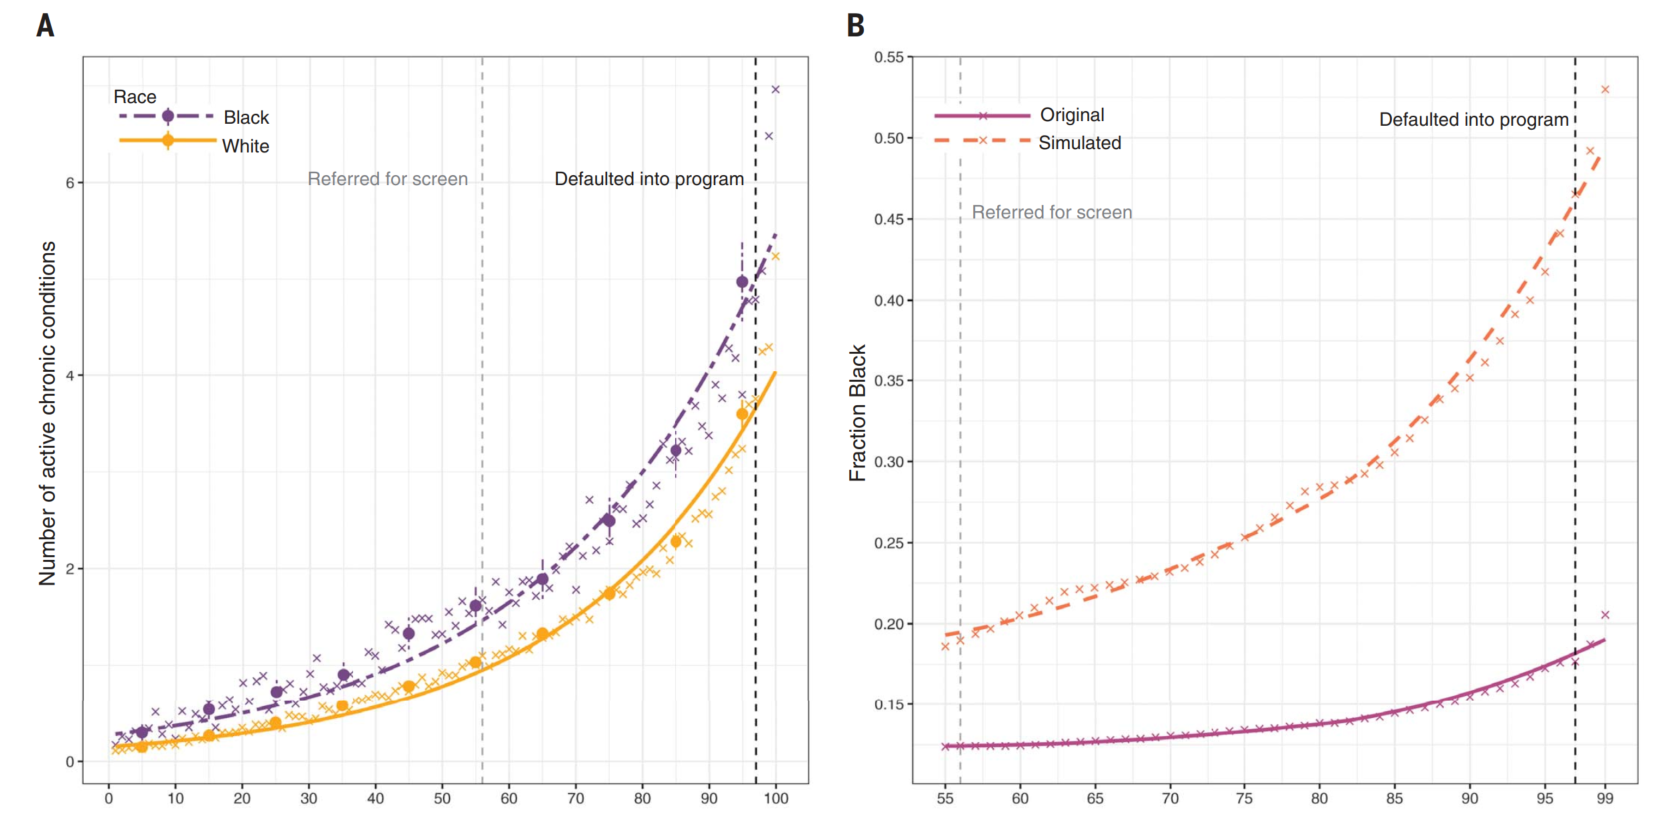
\includegraphics[scale = 0.4]{RiskPredictionAlgo1}
    \cite{OPVM19}
    \caption{In the left image: On each risk-level label, black patients are in a worse state than white patients. In the right image: Ziad Obermeyer, et al. introduce their prototype of a less biased version of the Risk assessment algorithm, it is an extreme change between the real and simulated scores comparing the 2 algorithms.}
  \end{center}
\end{figure}

How to quantify unfairness is a necessary step to approaching solutions.\cite{SHG*18} for that we need definitions appliable to the systems we are focusing in, which will be talked about in the next section. To efficiently repair the deficient part of a system we need to dissect it into the different parts that are sensitive to Biases. Dino Pedreschi et al. provide an interesting dissection of how a DSS, Decision Support System is built and the different "weak spots" for it to bend into not being fair and/or function properly at all. Please see Section \ref{ImplementingFairness} Figure:\ref{DSS}

\section{Mathematical Definitions: measuring (un)Fairness}
\label{mathdefinitions}
The following are classical and recent mathematical definitions which attempt to abstract the concept of fairness in different contexts. Either for the controlling of outputs of certain algorithms, or for generative solutions.\\
Two basic \textsl{frameworks} for measuring unfairness are:
\begin{itemize}
  \item Discrimination at an individual level
  \item Discrimination at a group level
\end{itemize}


\subsection{Individual Fairness}

\subsubsection{$\alpha$ Individual Fairness}\cite{DIJ20}
For a universe of individuals $U$, and a Metric $D:U\times U \to [0,1]$ for a classification task $H$ with an outcome set $O$, and a distance metric $d:\delta (O)\times \delta(O) \to [0,1]$, where $\delta(O)$ refers to the distribution over Outcomes of (O), and a randomized classifier $H:U\to \delta(O)$ is $\alpha$ individually fair, if and only if:
 \[\forall u,v \in U, d(H(u), H(v)) \leq\alpha D(u,v)  \]
"Similar individuals are treated similarly", this condition is based on the Lipschitz condition. And is thought to approach cases where the characteristics of the individual justly define the outcomes of a classification $H$, e.g: just students with a high-school diploma can apply to university. On that ground, individuals with similar characteristics should be treated equally. This of course has the potential to minimize individual disparity \textsl{within a group}, but not group disparity, as this method would give the same range of individual fairness to both a subject with a lot of commodities, and one with scarce ones as long as they are both treated equally among the shared characteristics of their peers. This illustrates the importance to understand the problem to be approached and choose the appropiate tools for the implementation of fairness measures.

\subsubsection{Consistency score}:
\[ C_{ons} = 1-\frac{1}{Nk}\sum_{n}{|\hat{y_n} - \sum_{y \in {kNN(X_n)}}{\hat{y_j}}|}  \]
The consistency score compares a model’s classification prediction of a given data item $x$ to its k-nearest neighbors $ kNN(x)$. \cite{RYK*13}The data item "nearest neighbors" can be interpreted as the other people or variables in the data set which share the most characteristics with our focused individual. \\
The individual is treated "consistently" or equally to it's peers if the treatment is the same over the other nearest neighbors. This is similar to $\alpha$ Individual Fairness, with the difference that it works on "clusters" of people around the observed person. It consequently shares the sames problems, and observations stated in the previous definition.


\subsection{Group Fairness}
To define group fairness, we will introduce the following terms:
\begin{align*}
  &\textup{\textbf{h}: X} \to \{ 0,1\} \textup{ The decision, treatment, or otherwise classification that's being controlled for fairness between 2 groups} \\
  &\textbf{X} \in R^d:\textup{ Set of d labels based on which the Algorithm shall make the classification. These generally are individual characteristics, single description variables or quantified features} \\
  &\textbf{S}: \textup{Sensitive attribute, membership in the Minority / Discriminated group or otherwise} \\
  & \textbf{Y}\in \{ 0,1\} :\textup{ Target value, the best categorization, ideally absent of discrimination}
\end{align*}

 There usually is the assumption of a probability distribution $D$ over $X$ which should resemble the probability of evaluation, meaning from all possible $ X \in Population$ the distribution assesses which elements of the population are more prawn to be classified. An example of this would be a loan, on reality just a section of the population would apply for a loan. \\

As stated before, it is important to recall that neither does \textsl{individual fairness} satisfy \textsl{group fairness} nor \textsl{group fairness}  satisfies \textsl{individual fairness}.

\subsubsection{Statistical Parity}
\[bias_h(X,S,D) = P[h(x) = 1|x \in S^C] - P[h(x) = 1|x \in S] \]

A hypothesis $ h:X \to \{-1,1\}$ is said to posess statistical parity on $D$ concerning $S$ up to bias $\varepsilon$ if $|\textup{bias}_h(X,S,D)| < \varepsilon.$ \cite{Math15b}\\
So if a classifier $h$ achieves statistical parity, we can interpret it as both the protected group $S$ and the rest of the population treated $S^c$ having fairly equally outcomes adjusting on $\varepsilon$.\\ However, this concept, as well as all others recited in this listing isn't independent of flawed data\footnote{look at section Data Bias}. There is an important amount of trust in the data fed into the system to appropriately represent every group and individual. This is of course a rather utopic goal that should always stand as reference, highly flawed data has big impacts on the outcomes of the systems we are speaking of.



\subsubsection{Equal error rates}:\cite{21c}
Another type of unfairness can be to have a good/informed decision in one group, and poor/random ones in another, despite equal positive rates on other group fairness models. \\
It is usually a consequence of Majority Bias(subsection \ref{MajorityBias}), meaning one of the groups  represents a small proportion of the whole data.\\

This measures the rate at which both acceptance and rejection errors happen, where D is the true label.
$$P(h(x) = 0|D = 1, x \in S) == P(h(x) = 0|D ==1, x \in S^C)$$
$$P(h(x) = 1|D = 0, x \in S) == P(h(x) = 1|D=0, x \in S^C)$$
In some scenarios, this measure may be even more important than the measures described before. False positives in the health-sector have a much more harsh impact than a classification task for a recommendation system for example.\\ In practical situations, one should adapt the fairness goals for the project to the working definition that is going to be used in the model, given that as stated in various sections in this paper, fairness definitions often collide with one another.

\subsubsection{Four-fifth rule}:
The four-fifth rule is a measure for analysing adverse impact, typically used in law and human resources agencies. It is an intuitive and rather simple way to measure selection rates between 2 groups.\\
The Four-fifth rule states the following:
\begin{quote} "If the selection rate for a certain group is less than 80 percent of that of the group with the highest selection rate, there is an adverse impact on that group" \end{quote}
It is used as the first analytic step in many procedures in the United States since 1978 where it was promulgated via EEOC the Uniform Guidelines on Employee Selection Procedures.

\subsubsection{Fairness through Unawareness}:

This is a concept that relies on the idea that when developing a predicting model the developers understand the possible discrimination towards a set of people $S$ in comparison of the other part of the population $S^c$. In that case, they can decide to \textsl{ignore} the sensitive value (in this case the belonging to a group $S$) from the set of characteristics $X_i$ which encapsulates relevant data for the prediction.
\begin{quote}"A predictor is said to achieve fairness through unawareness if protected attributes are not explicitly used in the prediction process" \cite{GaPe17}\end{quote}
% (https://www.fatml.org/media/documents/formalizing_fairness_in_prediction_with_ml.pdf)

The problem with this approach is that there usually are many \textsl{highly correlated} features in the vector $X_i$ to the sensitive one. The living location of people would is a good example: Location is often highly correlated to the membership to a certain part of the population. Meaning, the removal of a sensitive attribute is not enough to reduce unjust outcomes, and usually replicates close to original results.

\section{Implementing Fairness}
Having found unfair results in a system means a retroactive measure is to be taken. In this case, the system should be appropriately analyzed to find the parts to be adjusted. The second approach is the implementation of fairness measures during the conception of a system, the actions are then proactive. The following are some classification for assessing unfairness in a decision-making system.
\label{ImplementingFairness}
\begin{figure}[h!]
  \caption{Reference Model for analyzing and Reasoning on Discrimination in DSS (Decision support system) \cite{PRT09}}
  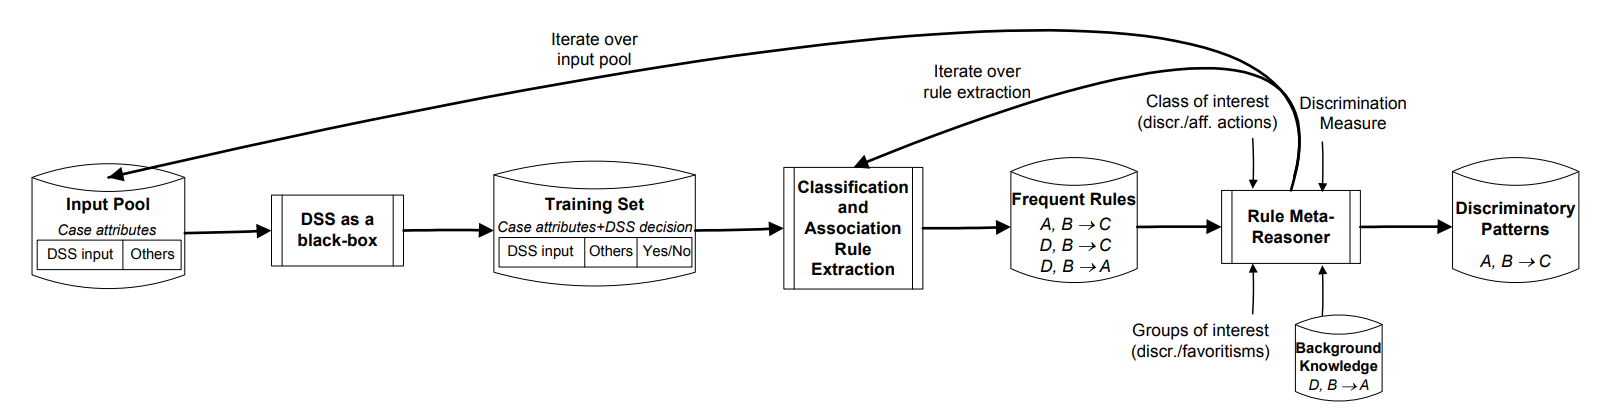
\includegraphics[width = \textwidth]{DiscriminationInDSS}
  \label{DSS}
\end{figure}
assessing unfairness comes from different stages.
\begin {itemize}
  \item Methodology to \textsl{detect} discrimination
  \item Methodology to \textsl{measure} discrimination
  \item Methodology to \textsl{avoid} discrimination
\end{itemize}
In Fig 2. we can appreciate a graphical model that intends to categorize the different stages that can be separately analyzed to encounter the source of discrimination in a DSS.\cite{PRT09}
\subsection{What do designers need}
Kenneth Holstein et al. conducted a survey in their paper "Improving Fairness in machine-learning Systems:
What Do Industry Practitioners Need?"\cite{HWD*19} in which they asked people involved in machine-learning development in the industry about the actual stand of "Fairness" in their place of work, the following concerns were found to be highly present.
"Needs for support in fairness-aware data collection and curation, overcoming team’s blind spots, implementing more proactive fairness auditing processes, auditing complex ML systems, deciding how to address particular instances of unfairness, and addressing biases in the humans embedded throughout the ML development pipeline". \\
This shows how concern in the academic world, and in the general public doesn't directly or as fastly translates to change in the industry and thus the touching points between the populations, and these products is not a direct patheay.


\subsection{Legal Regulation for Algorithms}
\label{legal}
A legal scheme to cover possible negative outcomes of algorithms that have high influence/contact with people would be a good measure to standardize and create outlines for future scenarios where discrimination is found. It would resolve also the inevitable comparations between different systems, and possible remorse attached to it, and leave a central standard to be met by all enterprises/developers, and systems. The challenge is then to encounter such a standard, fitting for all legislations, and that is able to constantly adapt to the new developments, and technologies.\\
Given that legal regulations are usually hard to apply in a global manner, the task would then reside on the regional governments to develop such legislatures. That in itself can be a problem for global products like a Youtube recommendation system which could adapt and exploit legal loopholes depending on the country the system is set in.\\
Regulation for some algorithms is already present. Some software and data processing systems, like algorithms used in ‘slot machines’ in Australia and New Zealand must, by government regulation, be “fair, secure and auditable” \cite{LWT*08}. Section 28b of the German Federal Law on Data Protection explains the necessity to have a scientifically proven statistical process to calculate the probability of a specific behavior of an individual before an algorithm can be used for making a decision about a contract.
Article 13 of the ECHR\footnote{European Commission for Human Rights} stipulates that "everyone whose rights, and freedoms as set forth in this Convention are violated shall have an effective remedy before a national authority" \cite{ECHR21}, having then found an active form of discrimination using the strategies, and protocols given on the earlier sections of this paper \nameref{discexamples}\nameref{mathdefinitions} it must be within the interest of each nation to address, and attend to a remedy for the wrong-doing. States must ensure individuals have the rightful opportunities to judicial procedures that will impartially come to a decision regarding their claims of violations of human rights.\footnote{This refers just to European nations, but the right no to be discriminated is also enlisted in the Human Rights act}\\
In the case of discrimination against protected groups legislation is very diverse, in Germany, the General Act on Equal treatment prohibits discrimination to six protected groups: \cite{20db} For the purposes of this paper we'll not include the playing definitions of Discrimination and Fairness in German Law, but they are to be found in 20db \footnote{Allgemeine Gleichbehandluchsgesetz} § 1, Section 2.
\begin{itemize}
  \item Race/ethnic origin
  \item Gender
  \item Religion of Belief
  \item Disability
  \item Age
  \item Sexual Orientation
\end{itemize}

In the end, it should be a shared work between the service giver and the user to seek potential problems in a product in order to minimize the negative impact on further usage of the product, together with the intervention of an independent sntitution that regulates outcomes of algorithmic decision-making systems.

\section{The Cost of Fairness}
Fairness implementations are restrictive measures in their nature, they serve as control for the outcomes of a system. A natural question that could arise is whether implementing fairness notions into algorithms have important pushbacks in efficiency, or even results?\cite{SHX05}\\
There can be a tradeoff between implementing fairness into a decision-making algorithm, and how efficiently the algorithm succeeds at its baseline job. The problem becomes ethical. Our society is not fair, and an algorithm that doesn't meet base standards of fairness promotes a disproportionate impact along social equality lines. It can even feed and increase social inequality.\cite{OBS*19} \\
Recent studies recite the holdbacks of implementing Fairness in Algorithms. The approach might "actually make the algorithm worse for everybody"\cite{Mill20}
even though the algorithm turns to be fair and equal in the outcomes to all groups using it. On their paper on "Algorithmic decision-making and the Cost of Fairness", Sam Corbett-Davies, et al. argue "Satisfying common definitions of fairness means one must in theory sacrifice some degree of public safety" \cite{CPF*17}, by common definitions of fairness they are talking about: \textsl{statistical parity, conditional statistical parity, and predictive equality}. \\
For each definition instead they propose thresholds that produce a decision rule that satisfies the fairness definition, detains 30 percent of the defendants, maximizes expected public safety.
They attempt to prove their posture empirically by deducting an Estimated increase in violent crime when fairness measures are used for the famous algorithm Chou16 covered in Section 2.
\begin{wrapfigure}{r}{0.6\textwidth}
  \begin{center}
    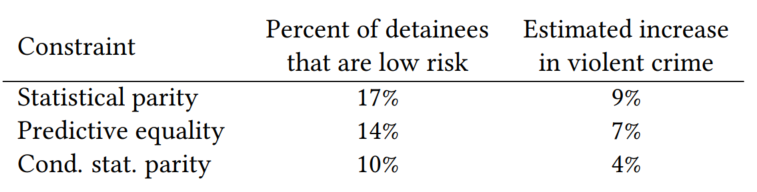
\includegraphics[width =0.6\textwidth]{Costoffairness1}
  \end{center}
\end{wrapfigure}

In the same paper, now from the other perspective, the cost of public safety results in a violation of all our working fairness definitions. From data from Brownley County: optimally detaining 30 percent of defendants meant 40\% of black defendants are detained, compared to 18\% of white defendants, and most importantly, among defendants who ultimately don't recede, 14\% of whites are detained compared to 32\% of blacks.\\

There is an inherent tradeoff between Fairness, and Utility. The goal of every system should be to develop a decision-making process that is \textsl{Non-Discriminatory}, while at the same time preserving quality of outcomes for the users.

\section{Contemporary implementation of Fairness Notions into Algorithms}
Now to understand the possible constructive power of algorithms in social-computing.
Although imperfect, at this time algorithms often tend to more accurately assess  even risk-based problems. \cite{Meeh13}\cite{GZL*00}\cite{Chou16}. Computer Science powered solutions have the potential to  provide an often difficult to reach neutral perspective of scenarios. They are also more easily scrutinizable and improvable. There is also the need to evaluate the negative symptoms of the presence of algorithms in decision-making positions; One of the most delicate setbacks being the inability of a deterministic system (the algorithm) to be subjective, and flexible to it´s context.\\
Another point in favor of the automatization of certain tasks is the understanding that human bias has effects up to, and especially at subconscious level; a way to avoid human bias is to automate the task, and let a "neutral" agent step in, let us denote that neutral is a sensitive word \footnote{In section Data Recollection the debate about how biased data impregnates machine-learning models is reviewed}
\subsection{A fair Recommendation System}
\label{RecommendationSys}
Recommendation systems influence which content is being shown in which order to consumers. As humans we are primed to follow rankings even without knowing what they are based on. Position Bias refers to disproportionately less attention being paid to low-ranked subjects, this phenomena leads to what is called the "Rich gets richer effect"; in the early stages of dynamic recommendation systems, when the first users are exposed to the content, the ranking is updated, which consequently affects the state of the ranking for the next batch of users who are then are affected by the Position Bias\footnote{The tendency to unconsciously infer the quality of a content based on the position they are on a ranking, or list.}, and this creates a snowball effect. The challenge is to find an algorithm that gives as equal as possible opportunity in all stages of the algorithm to the different types of content while maintaining a recommendation with high utility for the users.
\subsubsection{FairCo}
\label{FairCo}

Marko Morrik, Jessica Hong, Ashudeep Singh and Torsten Joachims consider the problem of dynamic Learning To Rank where rankings adapt based on users feedback. They present the first "dynamic LTR algorithm – called FairCo – that overcomes rich-get-richer dynamics while enforcing a configurable allocation-of-exposure scheme" \cite{MSHJ20}\\
\textbf{A naive Dynamic LeanToRank Algorithm}: \\
\begin{algorithm}[H]
\SetAlgoLined
Initialize counters $C(d)= 0 for each d \in D$\;
\ForEach{user}
{
  	present ranking $\sigma = argsort_D [C(d)]$ (random tiebreak)\;
    increment C(d) for the articles read by the user\;
}

 \caption{Naive Dynamic LTR}
\end{algorithm}

Content elements $d_i$ within this algorithm that get attention in the early iterations get a higher rank, and consequently more attention in the next rounds, which perpetuates the already described "rich get's richer" problem.

\textbf{LTR basics}:

For a set of Items $D$, a request  to the ranking system $$x_t , r_t \sim P(x, r)$$ is given, where $x_t$ is the users request of information and $r_t$ the user's vector of true relevance ratings for every item in the set $D$. The system then takes $x_t$ and dependant on a ranking policy $\pi_t(X)$ it produces a ranking $\sigma$ that is returned to the user. \\
After presenting the ranking $\sigma_t$ , the system receives a feedback vector $c_t$ from the user with a non-negative value $c_t(d)$ for every $d\in D$
The algorithm takes part in this step, where it receives the feedbacks $c_i$, the actual ranking $\sigma_i$ and the requests $x_i$ and computes the new ranking policy $  \pi_{t+1}(X)$:

$$\pi_{t+1} \gets A((x_1, \sigma_1, c_1), ..., (x_t , \sigma_t , c_t ))$$

\textbf{Evaluation of Ranking Performance}:

\[U^{DCG}(\sigma|r) = \sum_{d \in \sigma} \frac{r(d)}{log_2(1+rank(d|\sigma))}\]

This measures how good the ranking is based on the utility for the users, in which $r(d)$ stands for the relevance in the ranking of the item $d$.\\
The paper's definition of fairness for a recommendation system is an equal amount and quality of exposure for all the items in the query. To bind the concepts of merit and exposure they define:
\[Merit(G_i) = \frac{1}{|G_i|} \sum_{d \in G_i} R(d),Exposure_\textsl{t} (G_i)  = \frac{1}{G_i}\sum_{d \in G_i} p_\textsl{t}(d) \]
\[ R(d) = \int \textbf{r}(d) \,dP(\textbf{r}|\textbf{x}) \]
Where $R(D)$ is the expected relevance of the item d dependent on the request x. $p_t(d)$ is a position bias model \footnote{There currently exist several approaches to estimating such a parameter },  P is a probability distribution of requests, and $G_i$ denotes the group-content\footnote{this represent any categorization of any type of content, it is the way the items are organized to be analyzed for a fair representation} $i$ we are conditioning on.


The embedded definition of disparity within the model is: \\

\[ D^E_\tau (G_i,G_j) = \frac{\frac{1}{\tau} \sum_{t=1}^{\tau} Exp_t{G_i}  }{Merit(G_i)}  -   \frac{\frac{1}{\tau} \sum_{t=1}^{\tau} Exp_t(G_j)  }{Merit(G_j)}   \] which measures how well amortized is the exposure of the different elements of our set over $\tau$ steps. The closer this value is to zero, the less disparity. The exposure metric can be changed for impact, or other concepts of reachability dependant on the context the developer is implementing for.


\textbf{The Fairness control}:\\
The fairness control works with a Proportional Controller (P-Controller). It is a type of linear feedback control system in which a correction is applied to the working variable proportional to the difference between the \textsl{desired value}, in our case fair distribution of either merit or exposure, and the \textsl{measured value}.

$$\forall G \in \textsl{G}, \forall d \in \textsl{G} : err_\tau(d) = (\tau -1) \underset{G_i}{max}(\hat D_{\tau-1}(G_i,G)) $$
The error term $err_\tau (G)$ is zero for the group that already has the
maximum exposure/impact. This makes for an "adaptable" item that can control the value of the error term. For items in the other
groups, the error term grows with increasing disparity
The algorithm is then settled as:
$$FairCo: \sigma_t = argsort_{d \in D}(\hat R(d|x) + \lambda err_\tau(d))$$

\begin{figure}[h]
  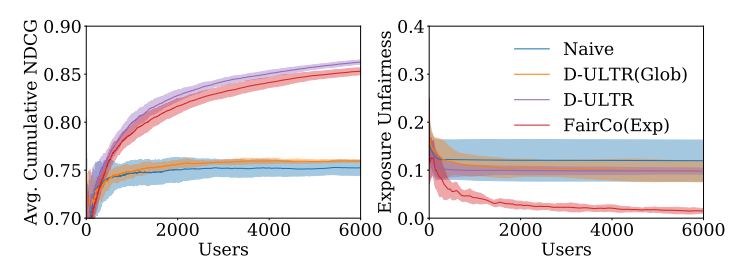
\includegraphics[scale = 0.8]{AverageExposureUnfairness+Users}
  \caption{A simulation of FairCo adjusted for Exposure against the Naive algorithm, and 2 common Ranking Systems online. NDCG is a usual measure for Utility.}
  \cite{MSHJ20}
  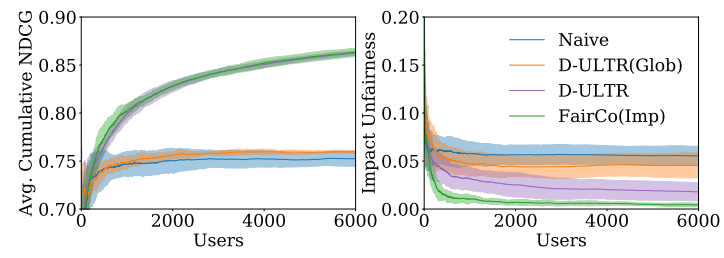
\includegraphics[scale = 0.8]{ImpactUnfairness+Users}
  \caption{A simulation of FairCo adjusted for Impact against the Naive algorithm, and 2 common Ranking Systems online. NDCG is a usual measure for Utility.}
  \cite{MSHJ20}
\end{figure}


FairCo is able to mitigate very strongly the rich-gets-richer effect among several contexts, while still achieving a high score of utility for the user. It is also left fairly open for the developer to  adjust the measure of utility, and Impact vs Exposure. The results are shown in the figures below.




\subsection{Division and the cake-cutting problem}
The division of resources is central to communal living, as such, it is also considered a sensitive subject that can bring disparity, conflict, and consequences on equality and equity.\\
The mathematical generalization of division problems is often known as the cake-cutting problem.\\
The repartition of goods is an activity that if not done well can lead to unfairness. It is an activity that is often studied by a lot of branches in the social sciences.\\
The simple question arises,"when do we consider a division to be successful?". Some of the most known ongoing approaches of the last years don't use keywords like fairness or equality. Instead, the central point is "envy-freeness". According to the Subjective Theory of Value, items cannot be given value in an objective manner, but rather are given a subjective value based on the "object's relationship to our needs"\cite{PrincEcon}. An envy-freeness approach is successful when all agents meet their subjective valuations. This paper would argue, that such a goal doesn't always enforce equality. The problem with the approach is that an agent feels envy-free if it's subjective valuation is fulfilled by the division. In real-world social applications, the paper suggests for the agents not to evaluate based on what they think they deserve, but out of an unbiased analysis, that suggests an impartial valuation and sometimes even an unjust one for oneself. Given the non-objective vision of humans, it is feasible to think that social agents can undervaluate, or overvaluate the subjective function. In that case, even an envy-free state would reflect an unfair, and unequal result.\\
The following are some implementations of division algorithms.
\subsubsection{Moving knife}\cite{Lang09}
The comparations now and further in the document will be based on the following theoretical assumptions.
The cake represents the goods to be divided as an interval $[0,1]$ , so the division is a partition $P_1,..., P_n$, where $P_i \in [0,1]$, $i \in (0,...,n)$.
The "knife" is moved from one extreme of the cake to the other. Any agent screams "stop" when it feels that from the actual position of the knife to the left there is $1/n$ of the value of the cake. In that case, the knife stops moving and the agent receives the section on the left side from the knife.
\begin{algorithm}[H]
\SetAlgoLined
\KwResult{Cake is divided in n sections}
totalCuts = 0\;
s = 0\;
\While{totalCuts <= n-1}
{
  	moveKnife()\;
    \If{$Participant_i$.screamsStop}
       {
       $Participant_i.piece = (s,actualPosition)$\;
       s = actualPosition\;
       totalCuts ++\;
       }
}

 \caption{Moving Knife}
\end{algorithm}

One of the weaknesses of this algorithm is that it depends on the truthfulness of the participants to scream exactly when they feel the value is correct. The other one is that it leaves space for abuse if some of the participants are not fast enough to react, as well as being prone to bad valuations of oneself's deserved piece of cake as stated before.


\subsubsection{Divide and conquer}
Every participant sets a flag on their middle, then recursively the middle is set by dividing the flags in the middle until there are just two parts, where each one then receives one part.
\begin{algorithm}[H]
\SetAlgoLined
\KwResult{Cake is divided in n sections}

$Flags \gets f_1,...,f_i$ \;
\ForEach{$Participant_i \in P$}
  {
  setMiddleFlag($f_i$)\;\tcp{Participants set the flag in what they think is the middle}
  }
$middleCut \gets argsort(Flags).median$\;
\If{|P| == 2}
{
  $participant_1.piece \gets [0,middleCut]$\;
  $participant_2.piece \gets [middleCut,1]$\;
}
\Else
{
  DivideAndConquer($[0,middleCut], Participant_1,...,Participant_{(n-1)/2}$)\;
  DivideAndConquer($[middleCut,1], Participant_{(n-1)/2+1},...,Participant_n$)\;
}

 \caption{Divide and Conquer}
\end{algorithm}

This algorithm is clearly inspired by the concept of divide and conquer present in other areas of computer science. It is also therefore very efficient. In the comparison in Fig 5. we are able to see this is the version that offers the least residing envy over all the other classical division algorithms. This is because, among other things, because participants are not in a real-time exercise like in the "Moving knife" algorithm thus there is no reaction time in the game.\\
This algorithm also offers a possibility to reevaluate the $valuation$ variable dependant on the outcomes of the previous iteration. even though this is also not an algorithm that can be envy-free in every situation, it is one of the best options.
\begin{figure}
  \begin{center}
    \begin{minipage}[b]{0.4\textwidth}
      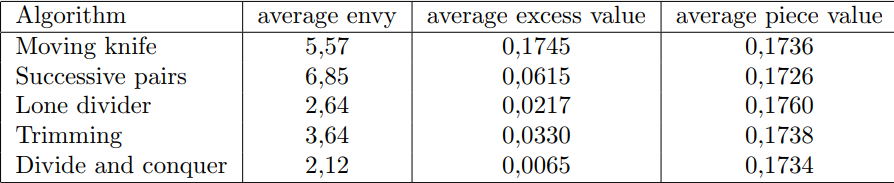
\includegraphics[width =0.8\textwidth]{ComparingDivAlg}
      \caption{Here is a comparison result of a simulation of different division algorithms, not only does Divide and Conquer offer the least amount of envy, it also has the less excess values for each division}
      \protect\cite{Lang09}
    \end{minipage}
    \hfill
  \begin{minipage}[b]{0,4\textwidth}
    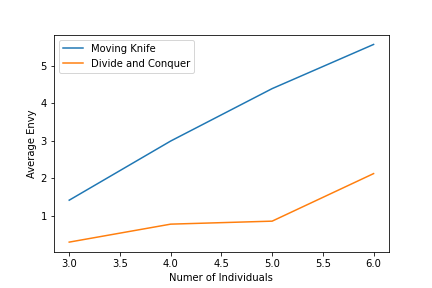
\includegraphics[scale = 0.4]{DivisionAlgComparison}
    \caption{Changing the number of agents taking part in a division, at least on the metric of envy Divide and Conquer offers better results \cite{Lang09}}
  \end{minipage}
  \end{center}
\end{figure}





% \begin{wrapfigure}{r}{0.5\textwidth}
%   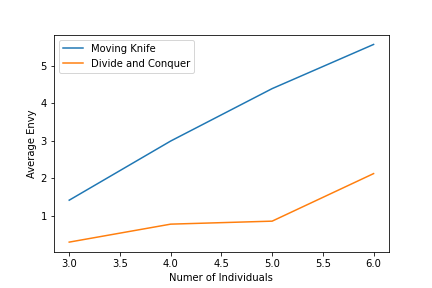
\includegraphics[scale = 0.4]{DivisionAlgComparison}
%   \caption{Changing the number of agents taking part in a division, at least on the metric of envy Divide and Conquer offers better results \cite{Lang09}}
% \end{wrapfigure}

\subsection{Fair Classifier and the move from division}
In situations like a distribution of clients asking for a loan, where the outcomes are binary, the cake division approach stumbles. As a response, other approaches improve the concepts of statistical fairness like the one described in the Section: Division and the cake-cutting problem where the usual variable is envy and the goal is a system that delivers as close a envy-free division as possible. Hossain et al. propose a different calculation of envy\cite{FairClassifier}. For a couple of groups
$G,Gb \subseteq X+$, and a dataset $S \subseteq X+$, and $\epsilon \geq 0$, we say that classifier $h$ is empirically $\epsilon$-Group envy-free on $G, \hat G$ with respect to S if:
\[ \sum_{x^+ \in S^G , \hat x^+ \in S ^{\hat G}} \frac{1}{|S^G|*|S\hat G|} %u(x+,h(xb)) − u(x+,h(x))
u(x^+, h(\hat x)) - u(x^+, h(x))\leq \epsilon\]  $$ S^G_i = S \cap G_i$$\\ This is similar to Statistical Parity, but in this case, the $u$ is the utility function for the user, which should describe the value for the user out of the given the classification $h$. It is normalized as $u: X^+ \times H \to [0,1]$
The idea can be adapted to further concepts like "Group Equitability"\footnote{In this version the 2 groups have \textsl{exactly} the same utility equity}
Formally the goal of Hossain et al. in the paper was to train a Model to learn a Mixture of:
\[\sum_{t=1}^{k} \eta^t h^t_d(x) \in \Delta^k(H) \]
 $\eta = (\eta^1,...,\eta^k) \in \Delta^k$, where $\Delta^k$ is the k-simplex that contains probability distribution for k elements in our data, and $h = (h^1_d,...,h^k_d) \in H^k$ is a family of multiclass classifiers, and we find the pair by minimizing a loss function that represents how fit the classifier is:
\[\underset{h \in H^k, \eta \in \Delta^k}{min}\sum_{t = 1}^{k} \eta^t \sum_{x^+ \in S} l(x^+, h^t_d(x)) \textup{  such that  } \forall(G,G^i) \in G :\]

\[\frac{1}{|S^G||S^{G^i}|} \sum_{t = 1}^{k} \eta^k \sum_{x^+ \in S^G, \hat x \in S^{G^i}} u(x^+, h^k_d(\hat x) - u(x^+,h^t_d(x)) \leq 0 \]

for group-envy-freeness

\[\frac{1}{S^G}\sum_{t=1}^{k} \eta^t \sum_{x^+ \in S^G}u(x^+, h^t_d(x)) = \frac{1}{S^G}\sum_{t=1}^{k} \eta^t \sum_{\hat{x^+} \in S^G}u(\hat{x^+}, h^t_d(\hat{x}))  \]

for group equitability\\
The loss function $l$ is originally the difference of the classification from the ground thruth in the fitting stage, but can also be implemented to different utility metrics for the users or the classifier.
\begin{figure}[h]
  \centering
  \begin{minipage}[b]{0.35\textwidth}
    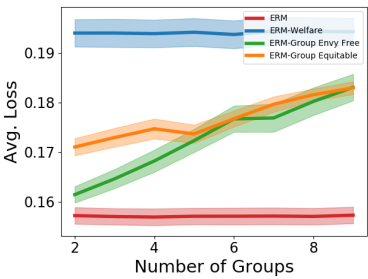
\includegraphics[width=\textwidth]{NumberOfGroupsFairClassifier1}
    \caption{Simulation of the fair classifier adjusting for \textsl{Loss} for the different fairness definitions, and no fairness definition}
    \cite{FairClassifier}
  \end{minipage}
  \hfill
  \begin{minipage}[b]{0.35\textwidth}
    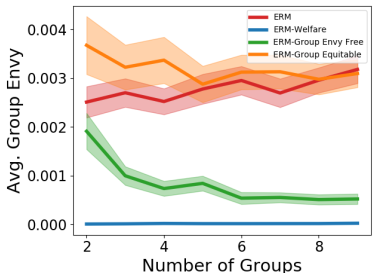
\includegraphics[width=\textwidth]{NumberOfGroupsFairClassifier2}
    \caption{Simulation of the fair classifier adjusting for \textsl{Envy} for the different fairness definitions, and no fairness definition}
    \cite{FairClassifier}
  \end{minipage}
  \centering
    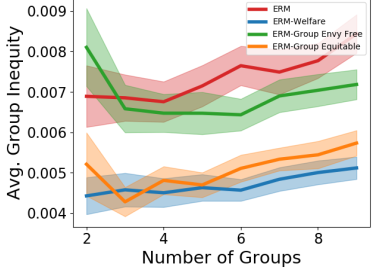
\includegraphics[width = 0.35\textwidth]{NumberOfGroupsFairClassifier3}
    \caption{Simulation of the fair classifier adjusting for \textsl{inequity} for the different fairness definitions, and no fairness definition}
    \cite{FairClassifier}
\end{figure}

This approach gives flexibility to the designer to define protected groups giving that it abstracts the problem to the pair of groups $G$ and $\hat G$. In the following figures we can appreciate a simulation from the researches based on different implementations of fairness notions, and a variable amount of protected groups.
\subsection{The human in the loop}
A lot of the measures described in the past chapters require solid and profound changes in education, legal system, protocols, training, and overall population awareness. Until then, correct practices from developers are needed. Supposing then a relative correct\footnote{a system which fulfills it's purpose without a concern for fairness for it's users} system:
An important question is the level of confidence in the autonomy of a non-human managing a system. The reachability of autonomy of a system is the in question.\\ This paper argues it is of moral responsibility, to constantly question and put a system on probation knowing the reach it has on people. Maybe more than a matter of confidence, it is a matter of giving importance to understanding the functioning of a human affecting entity. Therefore, a line of thought is to "keep the human on the loop". The agent then provides the neutral perspective while still accounting for human input in specific situations. This of course raises the predicament of defining these situations.
\subsection{Algorithms to avoid personal Bias, and conflicting notions of fairness}
There are various challenges to make the hiring of someone fair. Prejudice, Stereotypes, Bias, all controllable up to a point. Word, Zanna, and Cooper showed in their famous experiment of a Hiring Interview scenario \cite{WZC74} how prejudice creates negative expectations from the interviewer to the results of the interview, that influence the way the interview is directed and consequently how the decision is made, as well as establishing a pattern of Self-fulfilling prophecy for the job applicant. Self fulfilling prophecy is the term given to an effect in which an individual's expectations about another person or entity eventually result in the other person or entity acting in ways that confirm the expectations. In the case of the interview experiment, the people being interviewed actually performed worse based on the attitudes of the interviewer. \\
One of the challenges of any Human Resources department in an institution is to impartially assess  who to hire between a group of people interested in a job, putting individual and or group-prejudice, bias, preconceptions apart. Which can be very difficult to achieve.\\

Huysman, Sergeeva, et al. follow the task of the implementation of an A.I to automate the hiring process in a large multinational company. \cite{vSH19} \\
The initial motivation behind the implementation of the, in the paper called "NeuroYou" system, was to overcome the human risk of being biased against candidates, and to explore the potential to optimize the results of hiring. \\
NeuroYou worked by giving a series of tasks/games for the user to complete. "The neuroscience games aimed to measure cognitive (e.g. task-switching), social (e.g. assertiveness) and emotional (e.g. expression recognition) skills, and traits of participants in an easy-to-use interactive environment" \cite{vSH19} and giving a score based on the highest overlap of positive characteristics, and the statistical distribution of the results of the other participants. A score of 95 would imply that the candidate’s traits matched 95 percent of top-performing candidates, indicating a highly predicted successful employee at the company.\\
However, in later stages of the transition, once the system was giving scores to all candidates. (1) HR deviated from a fixed threshold, giving a chance of someone failing by 1\% (2) Managers tried and effectively challenged the "decisions" from the A.I\footnote{they challenged what otherwise would be a direct assessment from the A.I} (3) The team behind the software complained about the lack of consistency with the use of the system given that when ignoring the assessment the data going back into the system would be contaminated.\\
This is a very interesting example of how mathematical notions of fairness can clash with human and context based notions of fairness, and as the researchers also noted in their conclusion how the implemented system triggered a "negotiation" of ethical values. \\
In this case, it is arguable that even though the expected solution was not optimal, there was a healthy questioning of standards of fairness within the company, and further ethical values for the HR department.
\section{Discussion}
Establishing stronger standards for algorithms is necessary \cite{UNESCO18}, has very positive outcomes in respect to the effect on the users, but it can also affect the efficiency of development and even the algorithm itself . We need to find a control scheme, and apply it to all algorithms, especially on the stage of data recollection and analysis. Computer Scientists should have a social and ethical background to better understand the consequences of their work. This is not something new in other Areas of Technology and Science.\\
Algorithms should also be further investigated as tools to investigate social problems, of course with it's respective scrutiny.\\
A big point of collision in this discussion is the tradeoff between \textsl{utility} and \textsl{fairness}.It is highly arguable that the existence of the argument is in itself contradictory. Utility is a measure of how much \textsl{value} the user receives. The concept of fairness makes sure treatment among users is nondiscriminatory, or negative in any scenario. The discussion does not then stand behind utility, but pushing a gain in utility for specific users on the expense of other users.\\
Algorithmic approaches to the field of decision-making, division, recommendation systems, etc. are already being exploited and have big potential for improving conditions.
Finally, rigorous legal standards should be set on different levels to ensure the responsibility for the well functioning of these algorithms doesn't only reside in the developer's end, as well as for making legal battles in the area more transparent. Being treated by a fair algorithm should be a right.
\section{Conclusions, and Outlook}
Fairness in algorithms is in this time a very active sector, there are a lot of approaches, a lot of discussions, and new ideas; it is also an imperfect sector, one that being just in recent times in the spotlight, is still evolving, learning from mistakes, and \textsl{making} mistakes. As developers it is necessary to be more careful than usual with the errors to make, being conscious about how the outcomes of those errors have a heavy impact on real people.\\
Being careful doesn't necessarily mean decelerating the process of development, or innovation, but rather being more critical about it constantly in order to push to explore methods that would not be tried otherwise, due to the comfortability of the "easy solution".\\
While this discussion is not completely new to the Computer Science community, it is in its first stages in the Legal sector, and on popular knowledge. It is important to translate the concern for fairer algorithms to the general public. \\
Not only people, but algorithms gain from being fairer. Better Data recollection leads to better Models, better Data generation leads to better performance, better classifiers lead to a bigger, and \textsl{better} utility for the user.\\
Finally, as \cite{MSHJ20}\cite{FairClassifier} say, while their approaches offer some good results, they barely open the field of possibilities for future models, methods, and research.


% Bibliography
\bibliographystyle{../bibliography/ACM-Reference-Format}
\bibliography{../bibliography/bibliography}


\end{document}
